\chapter{Innovative SGT for the ASEAN economy}


\tab Following general considerations on the potential of SGT in chapter \ref{enhancing}, this chapter will present concrete areas of application of SGT in ASEAN. 

\vspace{0.4 cm}

This chapter will be divided in the following section:

\begin{enumerate}

\item A reminder of the general role and potential of SGT.

\item The presentation of key areas of application of SGT for ASEAN economy.

\item Finally, concrete recommendations based on the key areas introduced in section 2.

\end{enumerate}


\section{The role of SGT}

\tab As described in the previous section, SGT consists of four aspects:

\begin{enumerate}

\item \textbf{Real-time localization and tracking} of people, cargo and vehicles (air, sea, and land).

\item \textbf{Real-time monitoring of environmental and contextual information} covering all land and sea, such as: dynamic maps (traffic, congestion, people flow, and city changes) or environmental changes (weather, water and air quality, and greenery) from which events, accidents, and disasters can be extracted. Silent but meaningful changes such as climate changes and crustal deformation can be included.

\item \textbf{"Ubiquitous" data communications} at anytime/anywhere with small IoT devices to collect data from and to send instructions/guidance to people and machines in the field.

\item \textbf{High precision mapping} of 3D space and landscape framing activities of people and  autonomous vehicles/machines, while it could include very slowly moving phenomena like crust movement monitoring.

\end{enumerate}

For 1, it is technically possible to track most of all locational information of cars and people with the use of the wide-distributed smartphones. However, the collected data are often scattered, not shared nor even well exploited. Relating 4, Quasi-Zenith Satellite will start its full operation in 2018, and seven aircraft will be operated in 2023. Along with these developments, reinforcement service for high precision positioning such as MADOCA will be provided; and more accurate location information can be obtained. As a result, location information can be rapidly applied in various fields such as automatic driving and tracking of ground movement. Regarding 3, an integration of various information covering people and cars in mega cities, and interior areas including oceans and rural communities can be achieved with the help of IoT sensor networks and M2M communication networks developments. Indeed, "Oneweb", data communication service with global coverage with a large number of low altitude satellites, will provide a network on the whole earth by 20XX, and its implementation will be started by 2025. About 2, based on the PLANET and AXELGLOBE plans, typical emerging satellite observation companies deploying a large number of small satellites, real-time monitoring of the entire globe can be operated in 2025.

\vspace{0.4 cm}

These four principal functions are supposed to be implemented by 2025. Therefore, as described in the previous section, it is necessary to discuss the 2025 infrastructure strategy indicated by the MPAC, and its sustainability, toughness, and innovation of the ASCC blueprint associated with the current technological innovations.

\vspace{0.4 cm}

There are many common challenges in the ASEAN countries. For example, economic development and population growth are remarkable. Furthermore, there is a great potential for socio-economic developments resulting in excellent human resources developments. On the other hand, shortage of infrastructure investments, traffic congestion, environmental destruction, urban problems, and income disparity has been severely deepened.

\vspace{0.4 cm}

On the other hand, risks of natural disasters such as storms, floods, earthquakes, tsunamis, and landslides are very high; therefore, a huge investment is required for proper disaster managements. Transportation network developments connecting each country and socioeconomic developments cooperated by countries are still insufficient though investments of 16.6 trillion USD to road development will be needed by 2030 \cite{Dobbs2013}.

\vspace{0.4 cm}

SGT provides essential information for disaster response, expansion, and strength of international transportation networks, reduction of traffic congestion, optimization of logistic, comprehensive urban management, and strengthens the PDCA cycle.

\section{The expected contributions of SGT}

Among possible contributions of SGT, the significant contirbutions of SGT as solutions of social issues are summerized as follows.

\begin{enumerate}

\item Better Urban Development/Control including more sound financial basis
\item Better infrastructure planning and management incl. financing \item Better and safer, smoother Transportation Systems
\item Better Quality of Life by reducing cost and risks from disaster, accidents and diseases, and increasing job and financing opportunities.
\item Better Disaster Responses, Evacuation, and Recovery.
\item More efficient and secure Logistics.
\item More stable and profitable, safer and sustainable agriculture and fishery while conserving resources and environment
\item More efficient manufacturing and service industries supported by better logistics and micro-financing.
\item Better quantification and management of environmental services and national resources.

\end{enumerate}

\subsection{Better Urban Development/Control including more sound financial basis}

\tab Information such as stagnation and movement of people and vehicles, urban facilities developments, construction of houses, and infrastructures such as roads can be continuously provided by SGT; therefore, government and local communities can conduct proper policy making and monitoring aiming for urban planning, urban growth management and environmental improvement in an efficient way. For example, individual information on stagnation and movement condition of people and vehicles can be used for introducing new taxes such as congestion pricing and space use charge. Furthermore, extraction of buildings and land uses and their changes from satellite imagery can be utilized for strengthening building taxation, and land tax levies. To apply location information for taxation, it is necessary to implement a location authentication system to prevent spoofing.

\subsection{Better infrastructure planning and management incl. financing (road pricing etc.)}

\tab Infrastructural conditions can be timely detected through image analysis and sensor information; therefore, it contributes to preventing accidents caused by infrastructure damages and further to optimizing maintenance methods and timing of infrastructure. Real-time digital data of vehicles and people using transport infrastructure helps to improving optimization of infrastructure investment, and the overall optimization of infrastructure management including operation. For instance, an infrastructure usage-based charging system can be newly applicable; as a result, new resources and budgets for infrastructure management can be secured in addition to the better use of limited infrastructure resources. To apply location information for taxation, it is necessary to implement a location authentication system to prevent spoofing. Authentication can also be made possible using encrypted signal broadcasting from satellites.

Similarly, real-time supply and consumption of energy can be monitored as digital data; it also contributes to optimizing energy infrastructure operation and then investment, and finally leading to the overall optimization. Particularly in the field of renewable energy, where fluctuations of energy production are quite dominant, more detailed and reliable data on natural environments causing fluctuations can be obtained by SGT leading to the significant reduction in risks.

\subsection{Better and safer, smoother Transportation Systems}

\tab In the transportation system, SGT can track locations of vehicles, passengers, and cargo; therefore, it helps to real-time performance monitoring of transportation systems (smoothness, efficiency, and safety). SGT can easily detect problems and help continuously improvethe system in combination with performance monitoring. Furthermore, automatic operation and sharing of vehicles can be performed by using real-time positioning service, which dramatically improves efficiency and smoothness of the transportation system. Further, it provides a possibility to simultaneously improve uneconomical external factors such as traffic congestion, air pollution/noise, Greenhouse Gas (GHG) emissions. Also, improvements of traffic congestion greatly contribute to the improvement of productivities (e.g., service industry) by shortening traveling time in cities. Moreover, freedom of location (houses and shops) in towns can be significantly improved, enabling city expansion and improving competitiveness. To secure the safety of automatic operation, improvement of the security of positioning service will be really necessary.

\subsection{Better Quality of Life by reducing cost and risks from disaster, accidents, and diseases, and increasing job and financing opportunities}

\tab Collection and provision of real-time disaster information by SGT efficiently helps reduce disaster risks. It significantly contributes to improving Quality of Life (QoL) in Asia where disasters generate huge victims. Also, risks information such as traffic accidents and diseases can be provided as a temporal/spatial distribution so that these risks can be effectively reduced.  Outbreak of epidemic diseases could be better controlled with SGT, through monitoring people and patient movement together with environmental data to estimate the distribution of vectors like mosquitos.

Furthermore, collecting credit information for micro credit could be made easier and more reliable, providing an evidence of individual mobility pattern, social networks and mobile payment data. This system contributes to increasing employment opportunities, such as matching for temporary work. Also, the quality of life among people in terms of safety and income can be continuously traced and evaluated so that continuous improvement can be carried out through the PDCA cycle.

\subsection{Better Disaster Response, Evacuation and Recovery}

\tab The use of SGT helps quickly and exhaustively detect hazardous areas during disasters such as floods, landslides, earthquakes, and tsunamis. Therefore, evacuation can be promptly carried out in zones with a high level of risk, leading to the substantial reduction of possible damages. Moreover, the knowledge of the distribution and condition of evacuees facilitates the efficient provision of medical services and distribution of necessary items to the victims.

Furthermore, SGT allows to monitor post-disaster activities such as rebuilding or economic recovery of damaged areas. By performing continuous and detailed assessments of disaster response and recovery activities, it helps provide in a timely manner appropriate support at suitable stages. Furthermore, problems can be continuously discovered and solved through the PDCA cycle.

\subsection{More efficient and secure Logistics}

\tab The use of SGT enables to track movements of cargo, transportation vehicles and ships in real-time so that a reliable and continuous evaluation of transport and logistics performances can be made, leading to a significant reduction of the cost and duration of transportation.

In case of disasters and failures, logistical delays can be forecast; therefore, damages can be reduced by adapting production amount and its distribution process. Moreover, damages on roads can be detected in advance, so that delays and losses of logistics can be minimized by rearranging its routes and transport methods. By combining trajectory analysis and location verification, products’ deliveries to recipients can be confirmed, leading a secure logistics without theft or illegal sales during the process. Acquiring the detailed information such as route enables to better manage the quality of the products (e.g., refrigerated items and fragile objects). Furthermore, during transfer from a ship to a truck, automation of cargo handling machines using secured high-precision positioning service has been developed. This contributes to greatly improving efficiency and reducing cost and time during operation, especially considering a very large geographic range of the ASEAN.

\subsection{More stable and profitable, safer and sustainable agriculture and fishery while conserving resources and environment}

\tab In the industry of agriculture and forestry, use of SGT helps to understand about details of agricultural production systems including growing processes and crop management practices. It contributes to improving agricultural operations, reducing risks of productions, and improving/stabilizing productivities and profits. More importantly, accumulation of these data and integrating them into weather and market predictions can significantly contribute to risk reductions and production optimizations at a higher level. In addition, purchasing insurance can be further reduced possible risks. Governments and agricultural market personnel can reduce agricultural impacts by controlling market fluctuations through arranging stockpile and adjusting imports and exports based on the production forecasts. Furthermore, from the viewpoint of management of land and water uses, SGT can contribute to examining proper resource uses in agriculture (cultivation, products, water use) and in forestry. Necessary improvements can be carried out accordingly.

\vspace{0.4 cm}

In the industry of fishery, use of SGT enables to check detailed conditions of sea and fishing boat operations, estimate catch amount, and understand the status of fish resources and fish farm operations. This improves a fishery operation, reduces risks of production and maritime accidents, leading an improvement and stabilization of productivity and profits. Furthermore, entrance fees and charges/regulations on the basis of resource use can be applied in the operation, leading sustainable resource uses as well as ensuring funds for the resource management. Accumulating these data and integrating them with the predictions of sea, weather, and market can largely contribute to risk reductions and production optimization. In addition, purchasing insurance can be further reduced possible risks. Governments and marine product market personnel can reduce risks by controlling market fluctuations through arranging stockpile and adjusting imports and exports based on the production forecasts. Furthermore, from the viewpoint of fishery resources and coastal environmental management, SGT can contribute to examining proper resource uses in terms of operation and coastal area utilization (water quality management, topography modification, and protection of mangroves), and can be improved if necessary. To apply location information for developing charging system and regulation, it is needed to implement a location authentication system to prevent spoofing.

\subsection{More efficient manufacturing and service industries supported by better logistics, transportation systems.}

\tab Improved efficiency and safety of logistics and reduced distribution cost and transportation time lead reduction of production cost in manufacture, service, and construction industries. Furthermore, allocations of production bases and branches will be flexible; as a result, unbundling such as production, distribution, and consumption will be further promoted. Especially in the construction industry, uncertainties of procuring materials, equipment and labor force will be decreased, leading efficient process management and reduction of construction costs. As a result, arrangements of production and logistics bases will be further optimized in ASEAN countries; thus, management styles such as company size expansion will be more flexible. Improved traffic system will also facilitate the flow of people, expand one’s living area such as shopping and commuting areas, and easily attract tourists; as a result, it leads the expansion of the industries and revitalization of the regional economy. The competitiveness among ASEAN countries will be further improved.

\subsection{Better quantification and management of environmental services and natural resources.}

\tab Development of SGT enables to understand the details including amount and distribution of environmental services and natural resources in a quantitative way. This helps governments and companies to more rationally conduct decision-making by considering a balance among development, use, and conservation. In addition, as the use of environmental services and natural resources can be understood, countermeasures can be immediately taken against inappropriate uses. Furthermore, introducing a charging system further promote its appropriate usage. This process strongly secure financial resources for environmental resources management. Thus, sustainable and adequate environmental services and use of natural resources can be achieved through the system development.





\section{Concrete recommendations and examples of an efficient use of SGT}

\tab This section presents concrete recommendations for the application of SGT for the enhancement of ASEAN economy.

\subsection{Make cities smarter}

\begin{enumerate}

\item Better efficiency and effectiveness in taxation of land and fixed properties by monitoring constructions, vacant lands, and land uses from space.

\item Better and efficient of cadastral surveys provides basic information for taxations, such as land property.

\item 24/7 monitoring of urban transports (incl. passengers and cars) for choosing less congested routes and efficient transportations, minimizing confusions/congestions when events/accidents happen.

\item Charging car drivers and pedestrians for congestion time and places. In addition, charging road parking, street stalls, and disposals for controlling use of urban space and infrastructure. Then, increase of financial resource for urban management, while achieving more efficient uses of urban facilities/spaces.

\item Promotion of sharing economy by frequent (daily/hourly) monitoring of parking, office, and accommodations. Better efficiency in use of urban spaces.

\end{enumerate}

{\flushleft \bfseries Example: Urban applications of SGT in Nepal}

\begin{figure}[H]
\begin{center}
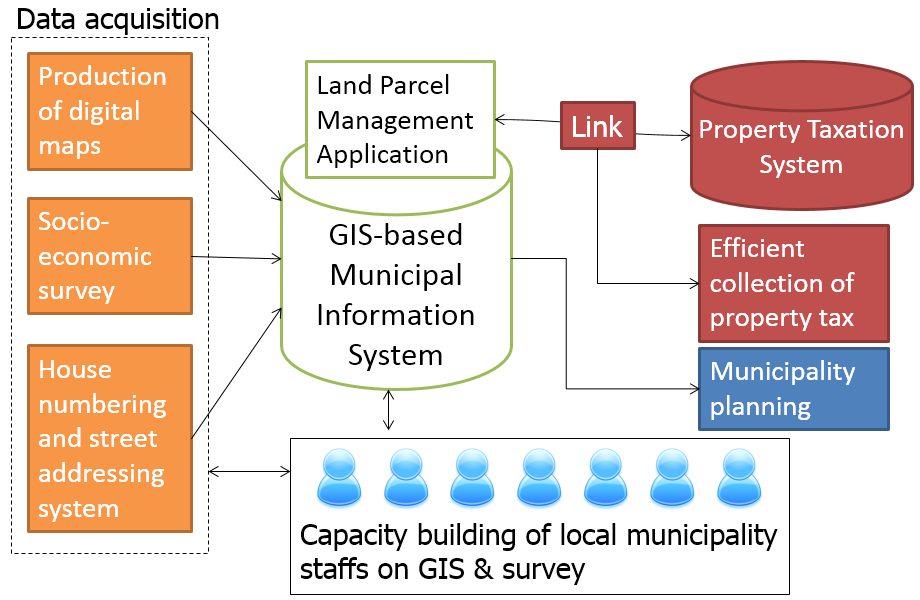
\includegraphics[width = 0.8\linewidth]{Figures/urban_nepal.png}
\end{center}
%\caption{urban_nepal}
\label{urban_nepal}
\end{figure}


\subsection{Improve the transportation sector}

\begin{itemize}

\item Significant improvement of management and operations by monitoring of both people/cargo movement and health of transportation infrastructure/vehicles.

\item Better safety by less incidents of transportation systems.

\item Reduction of disaster damages to transportation systems. Speedy evacuations of passengers and recovery of services

\item Data-driven, evidence-based planning of transportation infrastructure and healthy implementation of plans and operations.

\item Flexible adjustments of toll fees (road etc.) by location and time. Contribute to infrastructure development finance and better traffic controls.

\end{itemize}


\subsection{Improve the quality of life of people}

\begin{itemize}

\item Ensure people’s security by precisely delivered information about disaster and incidents.

\item Ensure epidemiological security by delivering precise risk information to people. 

\item Also provide health advices and information personalized by daily activities and exercises. These will improves efficiency of public health insurance.

\item Reduction of commuting time and traffic incidents by better traffic management. Safer and better quality of family life.

\item Better medical and health service efficiency by sharing location information of medical service resources, such as doctors, nurses, pharmacy, and instruments, in situations with limited resources.

\item More job opportunities and less unemployment rate by better job matching around home. And more safety by avoiding hazardous jobs by the better job opportunities.

\item Diverse education chances by various e-learning systems by ubiquitous network environments.

\item Promote community-based assistance through connections by location information and social media. This is very helpful in emergency responses.

\item Personal logs of activities and authenticated locations are utilized as proofs for individual authentication, anti-identity-spoofing and credit information of finances. It facilitates jobs of startups and small businesses via appropriate micro financing systems.

\end{itemize}


\subsection{Establish dynamic census}

\begin{itemize}

\item Nationally representative human mobility data with predicted demographic attributes

\item Advantages in data scarce environment

\item Safe-to-use because it is simulation data

\end{itemize}

\begin{figure}[H]
\begin{center}
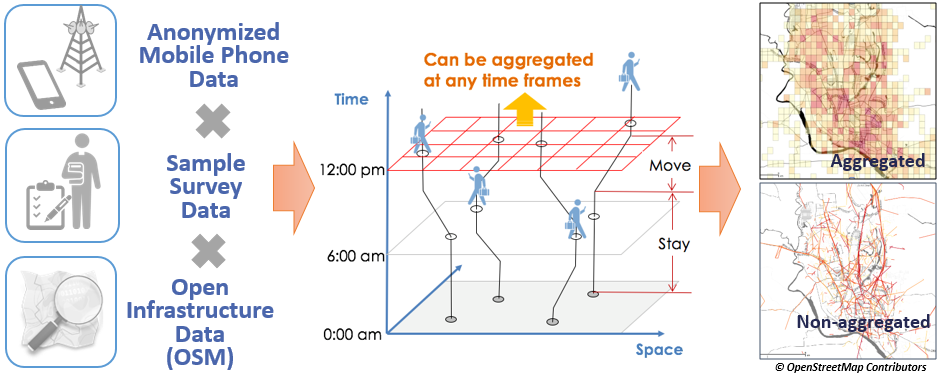
\includegraphics[width = 0.8\linewidth]{Figures/dynamic_census.png}
\end{center}
\caption{Schematic description of dynamic census}
\label{dynamic_census}
\end{figure}

{\flushleft \bfseries Example 1: Space-based Malaria Monitoring \& Control}

(Near) real-time mapping of malaria incidents and risks for decision support in malaria control by data collection, analysis, sharing, and visualization by combinations of space technologies and ground communications technologies. 

\begin{figure}[H]
\begin{center}
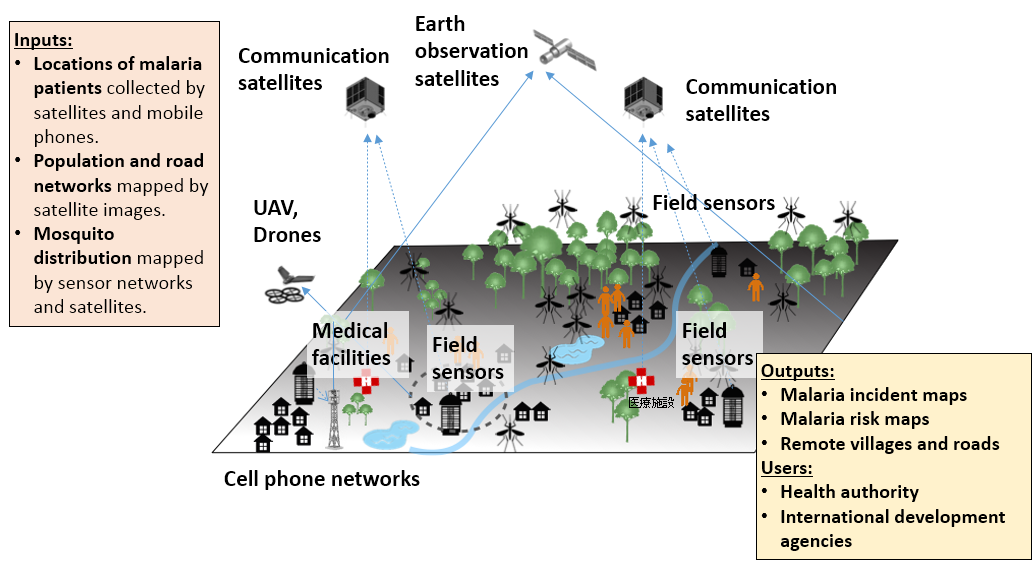
\includegraphics[width = 0.8\linewidth]{Figures/malaria.png}
\end{center}
\caption{(Near) real-time mapping of malaria incidents}
\label{malaria}
\end{figure}

{\flushleft \bfseries Example 2: People Monitoring for Ebola Control}

\begin{figure}[H]
\begin{center}
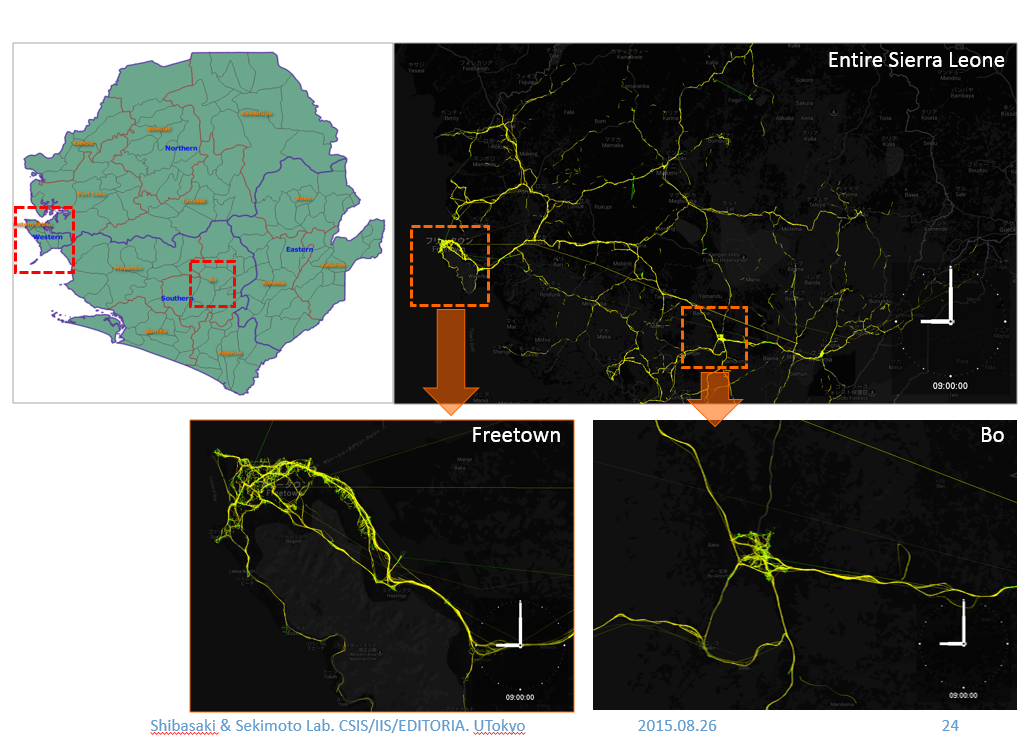
\includegraphics[width = 0.8\linewidth]{Figures/ebola.png}
\end{center}
\caption{People movement monitoring for Ebola control}
\label{ebola}
\end{figure}



\subsection{Enhance resilience}

\begin{itemize}

\item Reduce human damages by ensuring rapid information collection and delivery about disaster hazard and damages.

\item Ensuring goods delivery and debris removal by goods tracking and real-time recovery monitoring after disasters.

\item Higher accuracy of forecasts in ground/ocean weather information. Significant improvements are made using satellite earth observation. This provides industry and people  with lots of social benefits

\item By improving accuracy of monitoring and forecasting floods, slope failure, earthquake and volcanic eruptions, safety of people can be better secured.

\begin{figure}[H]
\begin{center}
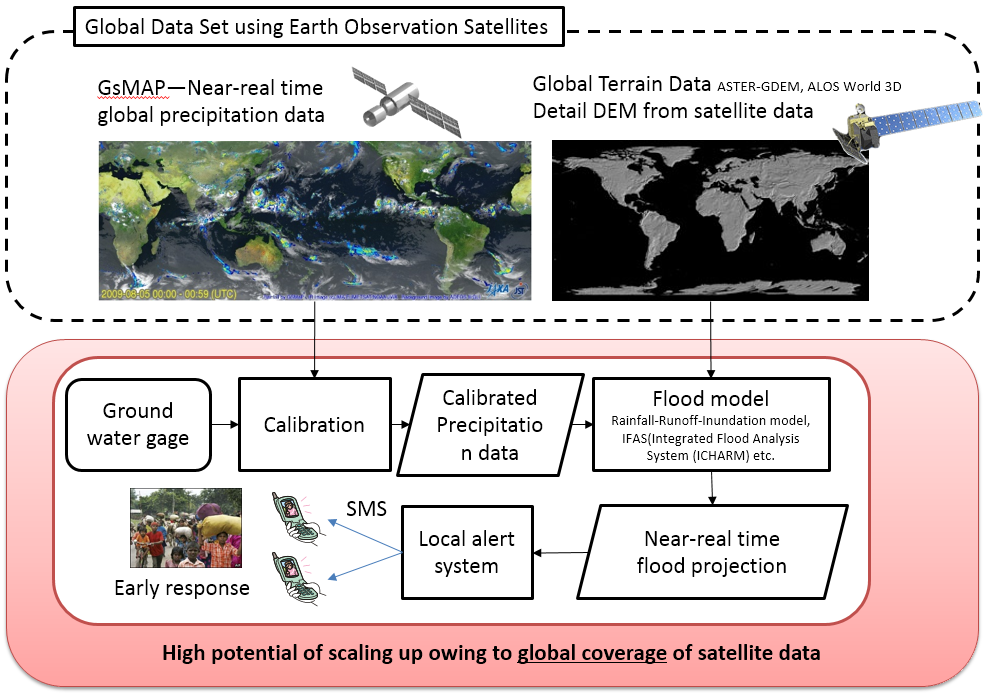
\includegraphics[width = 0.8\linewidth]{Figures/flood_alert.png}
\end{center}
\caption{Flood alert system with SGT}
\label{flood_alert}
\end{figure}

\item Disaster nursing supported with SGT.

\end{itemize}

\begin{figure}[H]
\begin{center}
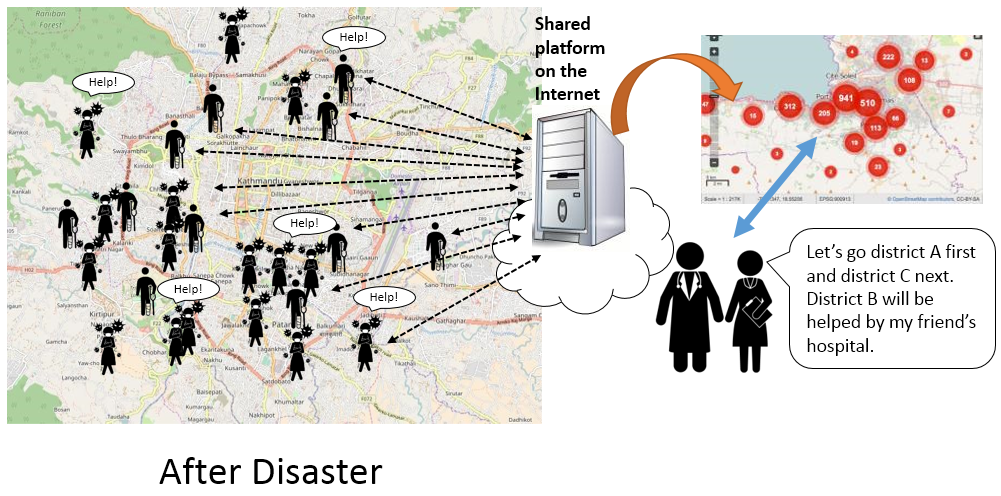
\includegraphics[width = 0.8\linewidth]{Figures/nursing.png}
\end{center}
\caption{Supporting disaster nursing with SGT}
\label{ebola}
\end{figure}

{\flushleft \bfseries Example: precipitation and flood monitoring in Bangladesh}

\begin{figure}[H]
\begin{center}
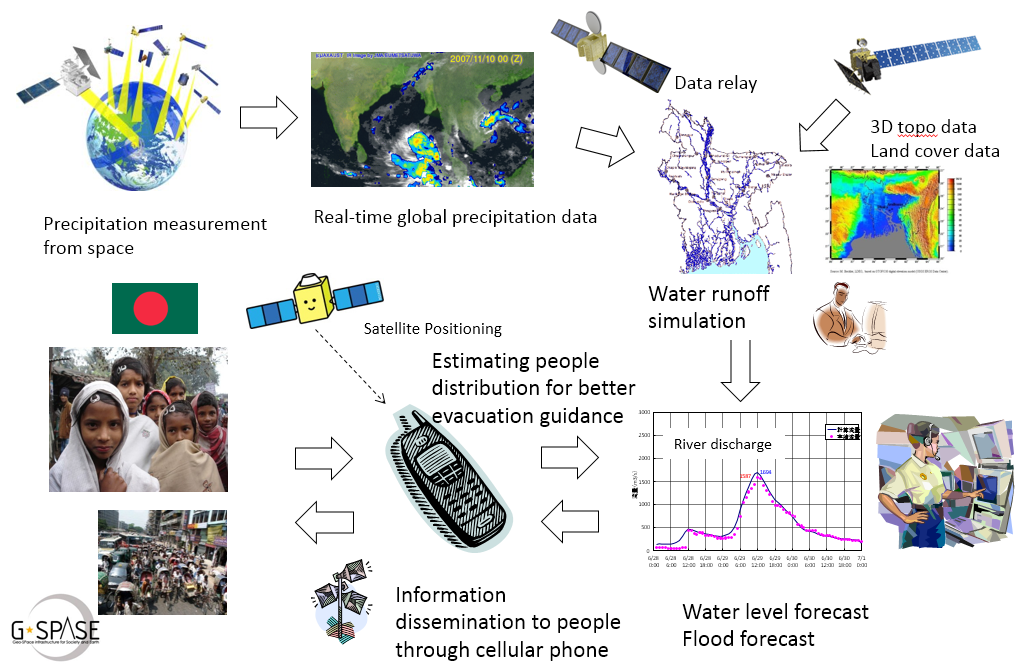
\includegraphics[width = 0.8\linewidth]{Figures/bangladesh.png}
\end{center}
\caption{Precipitation and flood monitoring in Bangladesh}
\label{bangladesh}
\end{figure}

\subsection{Improve logistics}

Track movement of things (cargos, freights) with authenticated position/time information, which enables:

\begin{itemize}

\item Certification of production place: more added-values by branding and safety, strengthening competitiveness and more activated industries and markets.

\item Less delivery loss and damages. Uber-like delivery service by average citizen. Smoother and cheaper logistic services. Strengthened logistic networks in remote areas, mountainous villages, and coastal areas.

\item More security and speed in custom clearance by certificates verified by authenticated mobility or location logs.

\item Securing collection, transport, and disposals of hazardous materials (e.g. industrial wastes) by movements monitoring. Contribute to environment conservation.

\item Reduction long-distance logistics cost by convoy transports of autonomous trucks on highways. ASEAN countries should have notable benefits owing to its dependency on road transports.

\item Much less operating cost and days by automation of container handling in harbors.

\end{itemize}

\subsection{Strengthen industrial activities}

\begin{itemize}

\item Agriculture

\begin{itemize}
\item Less damages by preparations to expected typhoons and hazardous weather, with adjusting timing of cropping, harvest, and shipping and so forth.
\item Optimized insurance cost by reducing agricultural risks and less compensation for agricultural damages from public sectors.
\end{itemize}

\begin{figure}[H]
\begin{center}
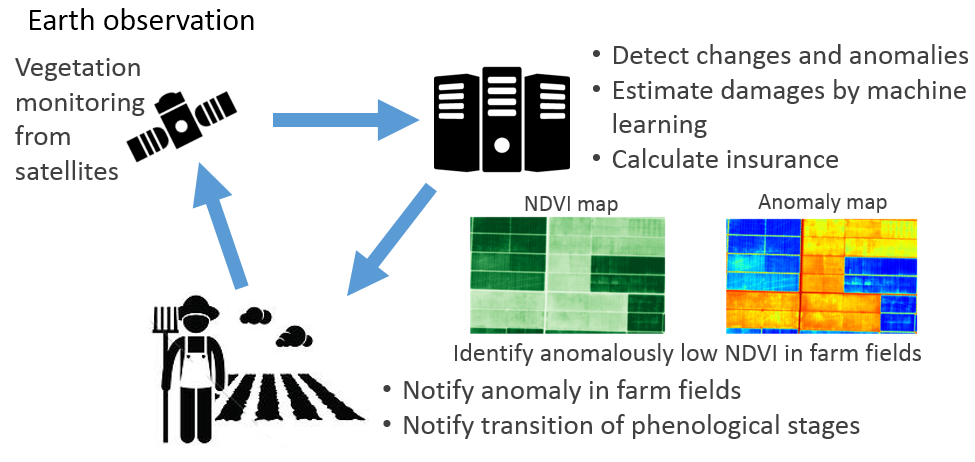
\includegraphics[width = 0.8\linewidth]{Figures/agri_anomaly.png}
\end{center}
\caption{SGT for agriculture}
\label{bangladesh}
\end{figure}

\item Fishery

\begin{itemize}
\item More efficient activities and operations of vessels and port facilities by forecasting harvestable areas and seasons. Better controlled market prices.
\item Less impact of oceanic hazards to fishery productions by meteorological forecasting. Better security by reduction of shipwreck. 
\item Better productivity and reduced disaster risks of aquaculture production by information of ocean condition and water quality (e.g. red tide).
\item Management of fishery resources, securing safe operations, and detection of suspicious vessels by tracking locations and operations of vessels with verified position authentication.
\end{itemize}

\begin{figure}[H]
\begin{center}
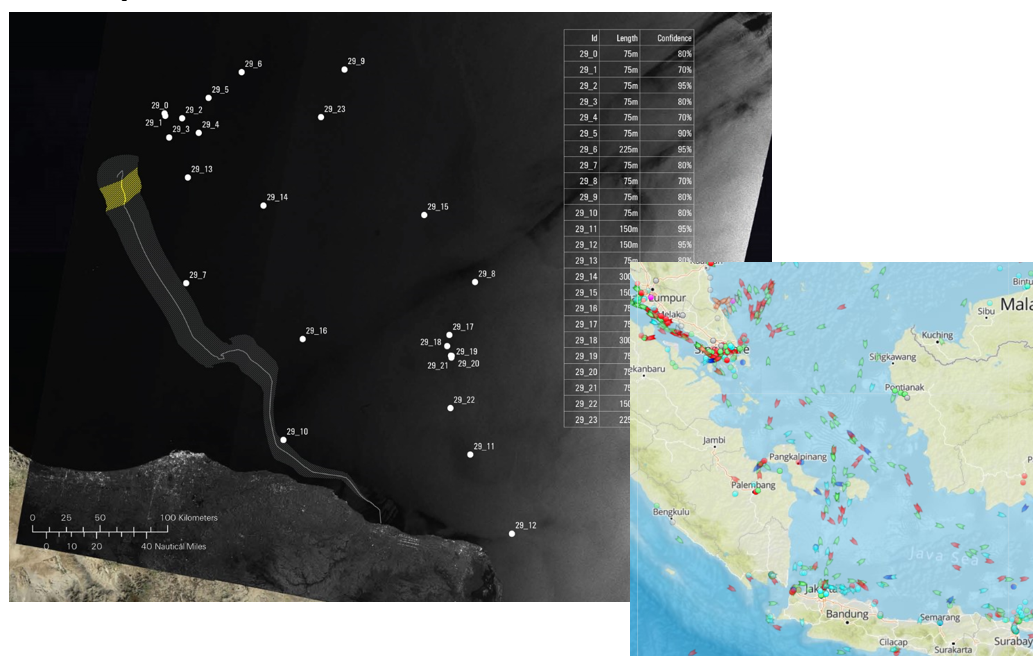
\includegraphics[width = 0.8\linewidth]{Figures/ship.png}
\end{center}
\caption{Unidentified ship detection by satellites and AIS/VMS}
\label{bangladesh}
\end{figure}

\item Forestry

\begin{itemize}
\item Ensure sustainable use of forest resources (planting, conservation, logging) by continuous monitoring of forest resources (biomass and tree types).
\item Better efficiency and effectiveness in logging, lumber, and transport by quantified planning of forestry operations. And less labor hazards.
\item Suppress damages of forest fire and illegal loggings.
\end{itemize}

\begin{figure}[H]
\begin{center}
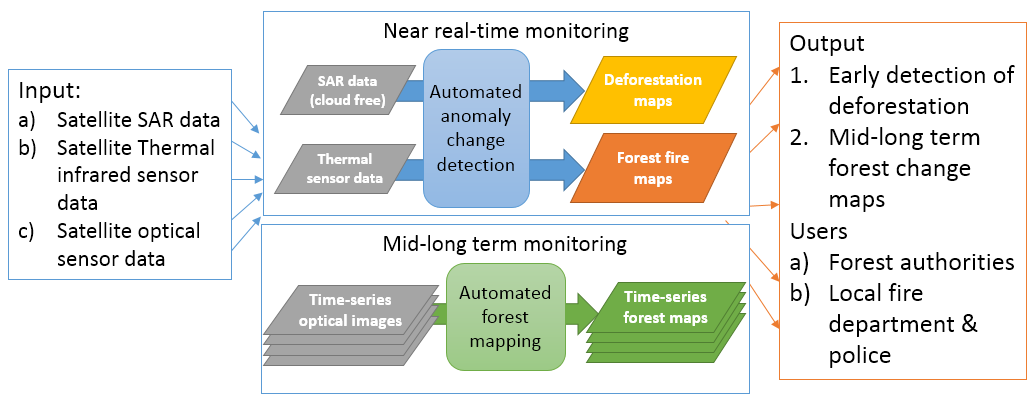
\includegraphics[width = 0.8\linewidth]{Figures/forest.png}
\end{center}
\caption{Forest monitoring with SGT}
\label{forest}
\end{figure}

\item Construction

\begin{itemize}
\item Risk reduction by effective designs and construction plans with accurately measured and shared data of terrain and geology.
\item Effective management of labors and staff safety with better efficiency of transports and stock usage by continuous and accurate monitoring of things and people’s position.
\item Quality assurance and improvement through detection and prevention of faults by accurate 3D measurement of construction progress.
\end{itemize}

\item Manufacturing

\begin{itemize}
\item Less logistics cost and uncertainty to deliver and procure products. Leading to cost reduction of manufacturing.
\end{itemize}

\item Service

\begin{itemize}
\item Less cost of service delivery by significant reduction of cost and uncertainty in logistics.
\item Realize possibilities of micro-consumer services, such as e-commerce and food delivery, by the low-cost and effective delivery services.
\item Better reliability of mobile payment using personal credit information based on locations and activities verified by positioning authentication. 
\item Scaling up of mobile micro consumer services by the more reliability of personal micro-payment systems.
\end{itemize}

\begin{figure}[H]
\begin{center}
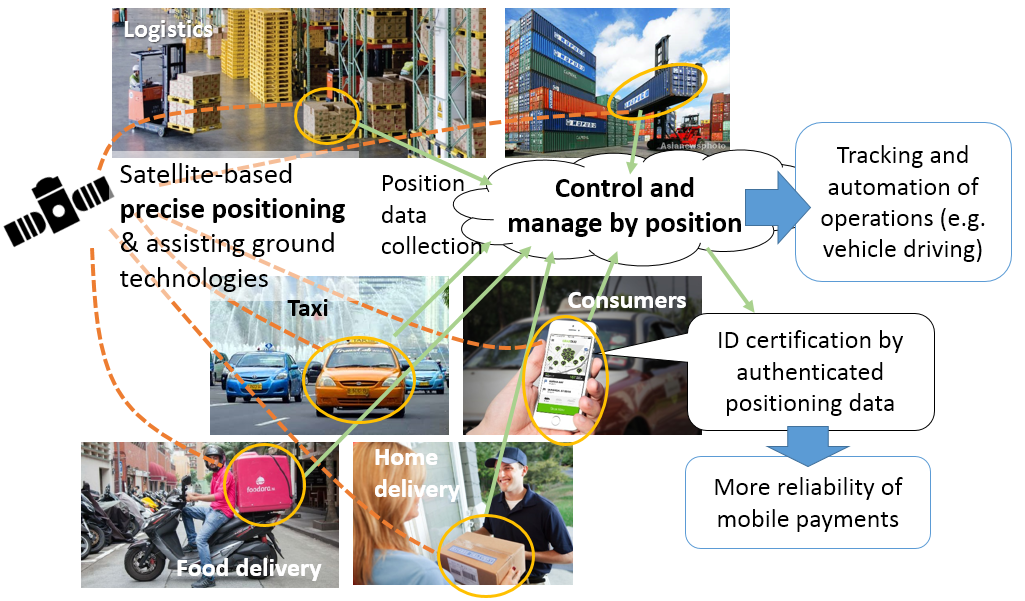
\includegraphics[width = 0.8\linewidth]{Figures/manufacturing_service.png}
\end{center}
\caption{SGT to support manufacturing and service sectors}
\label{manufacturing_service}
\end{figure}

\item Energy sector

\begin{itemize}
\item Energy demand and supply gaps visualized through satellite observations of city lights.
\end{itemize}

\begin{figure}[H]
\begin{center}
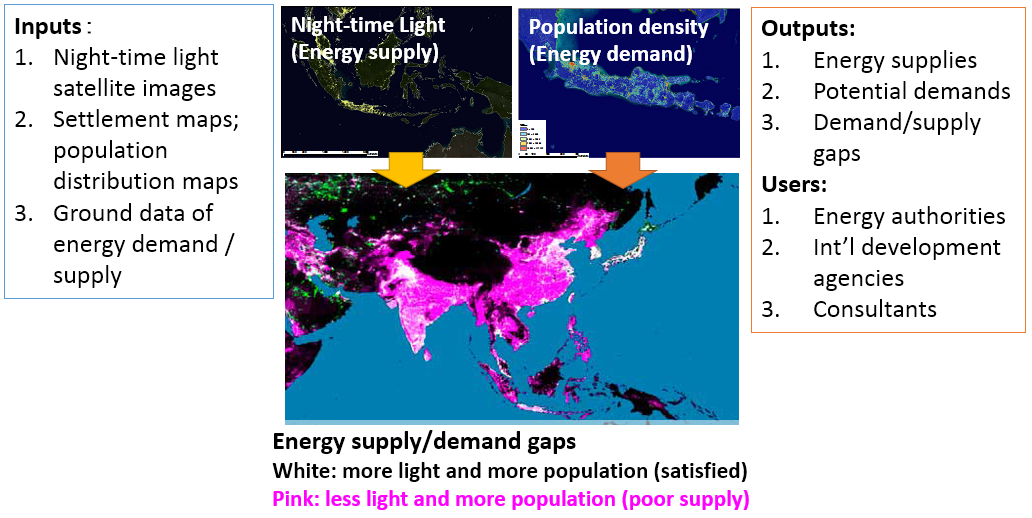
\includegraphics[width = 0.8\linewidth]{Figures/energy.png}
\end{center}
\caption{Estimating energy needs through night satellite observation}
\label{manufacturing_service}
\end{figure}

\end{itemize}

\subsection{Support environmental resources management}

\begin{itemize}

\item CO2 emission reduction by optimizing transport operations (taxi, commercial vehicles, and shipping vehicles) based on vehicle mobility data. This supports fund raising by environment finance scheme such as bilateral carbon offsets.

\item Effective conservation of ecosystem services by continuous monitoring of ecological status of forest, ocean, and marines.

\item Social bonds can be applied to better and sustain the services based on value evaluation of ecosystem services

\item Effective conservation and management of specific areas for species conservation and gene banks.

\end{itemize}

\begin{figure}[H]
\begin{center}
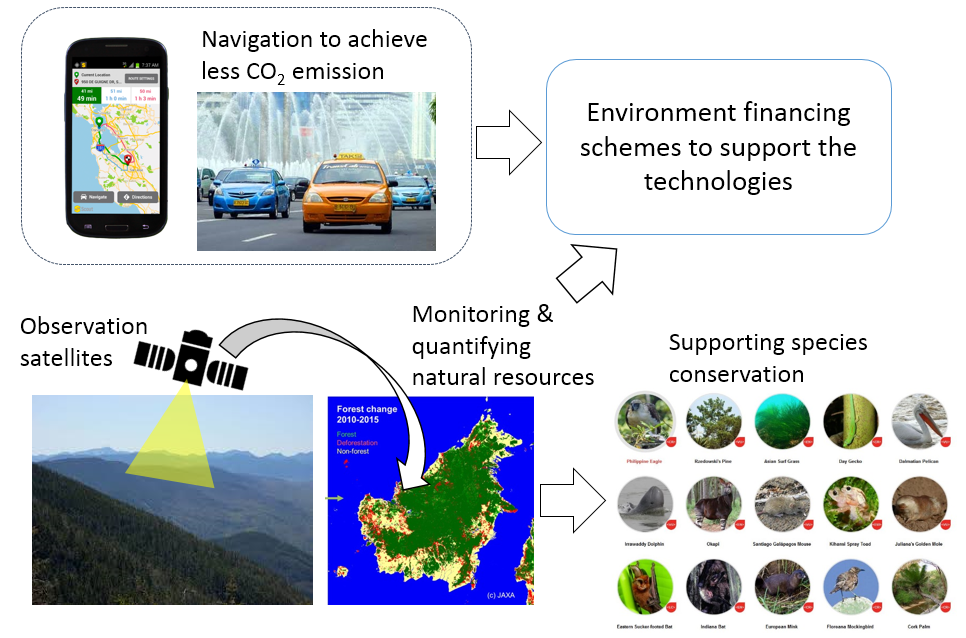
\includegraphics[width = 0.8\linewidth]{Figures/resource_manag.png}
\end{center}
\caption{SGT for environmental resources management}
\label{resource_manag}
\end{figure}

\subsection{Strengthen national land and sea management}

\begin{itemize}

\item Higher accuracy of forecasts in ground/ocean weather information using advanced satellite earth observation. This provides industry and people  with lots of social benefits.

\item Achieve marine safety and fishery resources conservation by strengthening detection and monitoring of unidentified ships.

\item Better safety/security of people by improving accuracy of monitoring and forecasting floods, slope failure, earthquake and volcanic eruptions.

\end{itemize}

\begin{figure}[H]
\begin{center}
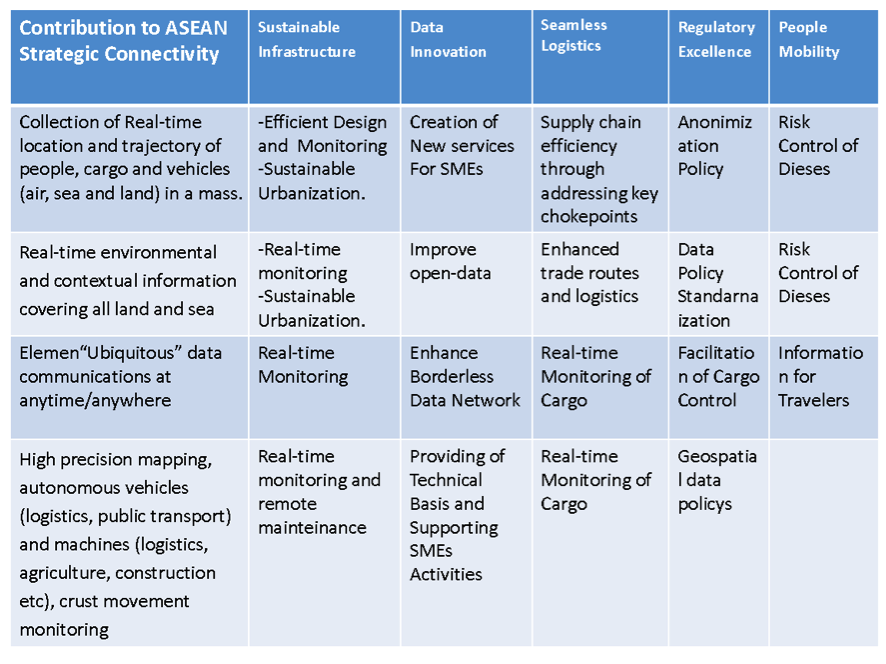
\includegraphics[width = 0.8\linewidth]{Figures/asean_connectivity.png}
\end{center}
\caption{Table asean connectivity}
\label{asean_connectivity}
\end{figure}



\section{Economic and industrial impacts -- Summary}

\begin{itemize}

\item Economic impacts of the improvement with SGT

\item Collecting examples...

	\begin{itemize}

	\item Traffic congestion

		\begin{itemize}

		\item Jakarta (Jakarta post 2015)
		
			\begin{itemize}
			\item 5 billion USD losses each year by traffic jam.
			\item 167 USD loss (person/year: 5\% of GDP per capita)
			\end{itemize}

		\item Nairobi, Kenya
		
			\begin{itemize}	
			\item 210 million USD loss each year 
			\item 60 USD loss (person/year: 5\% of GDP per capita).
			\end{itemize}

		\end{itemize}
	\end{itemize}
\end{itemize}

